\newpage
\section{Durchführung}
\label{sec:Durchfuehrung}
    Die Durchführung des Versuchs ist in drei Teile geteilt, zunächst werden im ersten Teil des Versuches die Moden des verwendeten Hohlleiters untersucht. Im zweiten Teil des Versuches soll die Frequenz, die Wellenlänge und die Dämpfung für die Mikrowellen bestimmt werden. Abschließend werden im letzten Versuchsteil stehende Wellen untersucht.
    \subsection{Versuchsaufbau}
        Um die für den Versuch notwendigen Mikrowellen zu erzeugen wird ein Reflexklystron (\ref{sec:Reflexklystron}) welches mit einer variablen Spannungsquelle versorgt wird verwendet.
        Nach der Mikrowellenquelle wird ein Einweggleichrichter platziert, welcher verhindert dass reflektierte Wellen in das Klystron gelangen.
        Nach dem Einweggleichrichter wird ein Frequenzmesser eingesetzt mit dessen Hilfe die Frequenz der Mikrowellen genauer bestimmt werden kann.
        Der Frequenzmesser besteht aus einem variablen Hohlraum mit dem der verwendete Hohlraumresonator modifiziert werden kann.
        Nach dem Frequenzmesser wird eine variable Dämpfung eingebaut mit der die Mikrowellen abgeschwächt werden können.
        Dieser Aufbau ist der Grundaufbau für die drei Versuchsteile, in den einzelnen Versuchsteilen werden verschiedenen Bauteile hinter die Dämpfung eingesetzt um die Messungen durchzuführen.
    \subsection{Untersuchung der Hohlleitermoden}
        Für die erste Messung wird hinter die Dämpfung lediglich ein Detektor angebracht welcher mit einem Oszilloskop verbunden wird.
        Der Detektor besteht dabei aus einer kleinen Nadel die in den Hohlraum ragt und als Dipol durch die Mikrowellen angeregt werden kann.
        \begin{figure}[H]
            \centering
            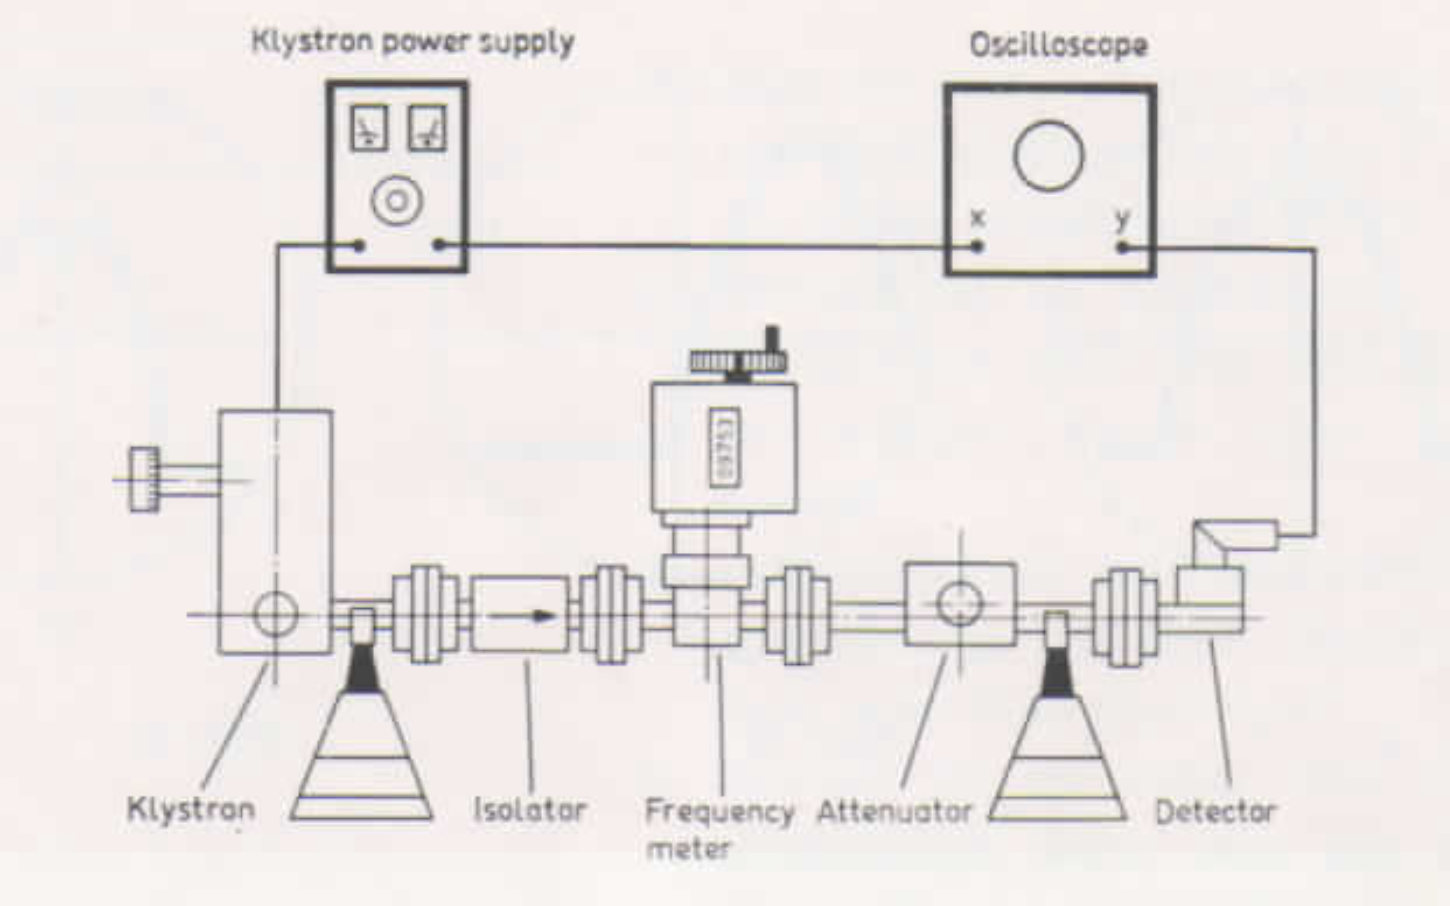
\includegraphics[width = 0.75\textwidth]{bilder/Aufbau_Teil1.png}
            \caption{Der Versuchsaufbau für die Untersuchung der Hohlleitermoden.}
            \label{fig:Teil1}
        \end{figure}
        Um die Moden des Hohlleiters zu untersuchen wird auf den x-Kanal des Oszilloskops die Betriebsspannung der Reflexklystrons und auf den y-Kanal die Spannung des Detektors gelegt.
        Mit dem Oszilloskop können dadurch die Moden sichtbar gemacht werden (\ref{fig:Moden-Abbildung}).
        \begin{figure}[H]
            \centering
            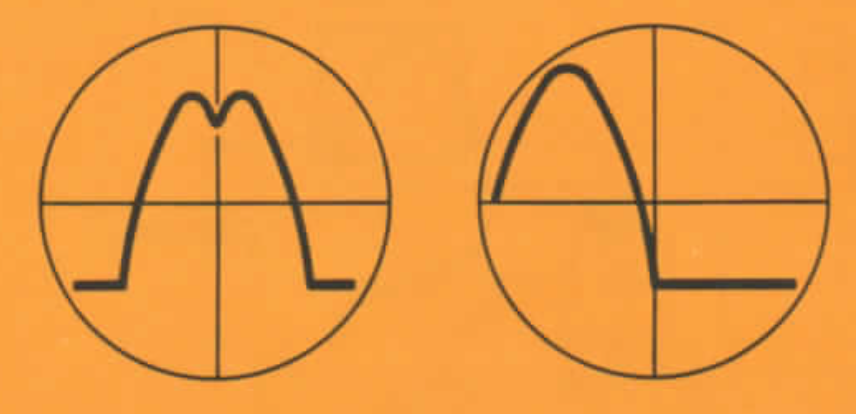
\includegraphics[width = 0.75\textwidth]{bilder/Moden-Abbildung.png}
            \caption{Moden-Abbildung.png}
            \label{fig:Moden-Abbildung}
        \end{figure}
        Die Reflektorspannung wird nun so gewählt, dass die Mitte der Mode mittig auf der x-Achse des Oszilloskops liegt.
        Nun wird der Frequenzmesser eingestellt um die Einbuchtung auf die Mitte der Mode und somit das Maximum zu bewegen und die Mittelfrequenz zu bestimmen.
        Von der Mode werden nun Mittelfrequenz, Reflektorspannung und Amplitude notiert.
        Diese Messung wird für zwei weitere Moden wiederholt und auch notiert.

        Anschließend wird für jede Mode noch die Punkte der halben Leistung vermessen indem jeweils rechts und links neben der Mode die Einbuchtung der Frequenzmessung auf den wert der halben Amplitude gebracht und die Frequenz sowie die Reflektorspannung notiert.
    \subsection{Messung von Frequenz, Wellenlänge und Dämpfung}
        Im zweiten Versuchsteil soll zunächst die Frequenz der Moden mithilfe eines SWR-Meters genauer bestimmt werden.
        Dafür wird hinter der Dämpfung eine Detektor für stehende Wellen und zunächst ein Abschluss eingebaut.
        Die Reflektorspannung wird so eingestellt dass ein Maximum am SWR-Meter erreicht wird während der Frequenzmesser verstimmt ist.
        Der Frequenzmesser wird anschließend so eingestellt, dass auf dem SWR-Meter eine Signalverkleinerung erkennbar ist und die entsprechende Frequenz wird notiert.

        Für den nächsten Abschnitt wird der Abschluss durch einen Kurzschluss ersetzt.
        Über den Stehwellendetektor werden die Positionen von zwei Maxima des SWR-Meters bestimmt und notiert um die Wellenlänge der Mikrowellen zu bestimmen.

        Abschließend wird der Kurzschluss wieder durch einen Abschluss ersetzt und eine Dämpfungskurve aufgenommen.
        Für die Aufnahme der Dämpfungskurve wird zunächst das SWR-Meter eingestellt, so dass es bei keiner Dämpfung einen Wert von \SI{0}{\decibel} anzeigt.
        Die Dämpfung wird weiter erhöht bis das SWR-Meter jeweils \SI{2}{\decibel},\SI{4}{\decibel},\SI{6}{\decibel},\SI{8}{\decibel} und \SI{10}{\decibel} anzeigt und die entsprechenden Einstellungen des Dämpfungsgliedes werden notiert.
        \begin{figure}[H]
            \centering
            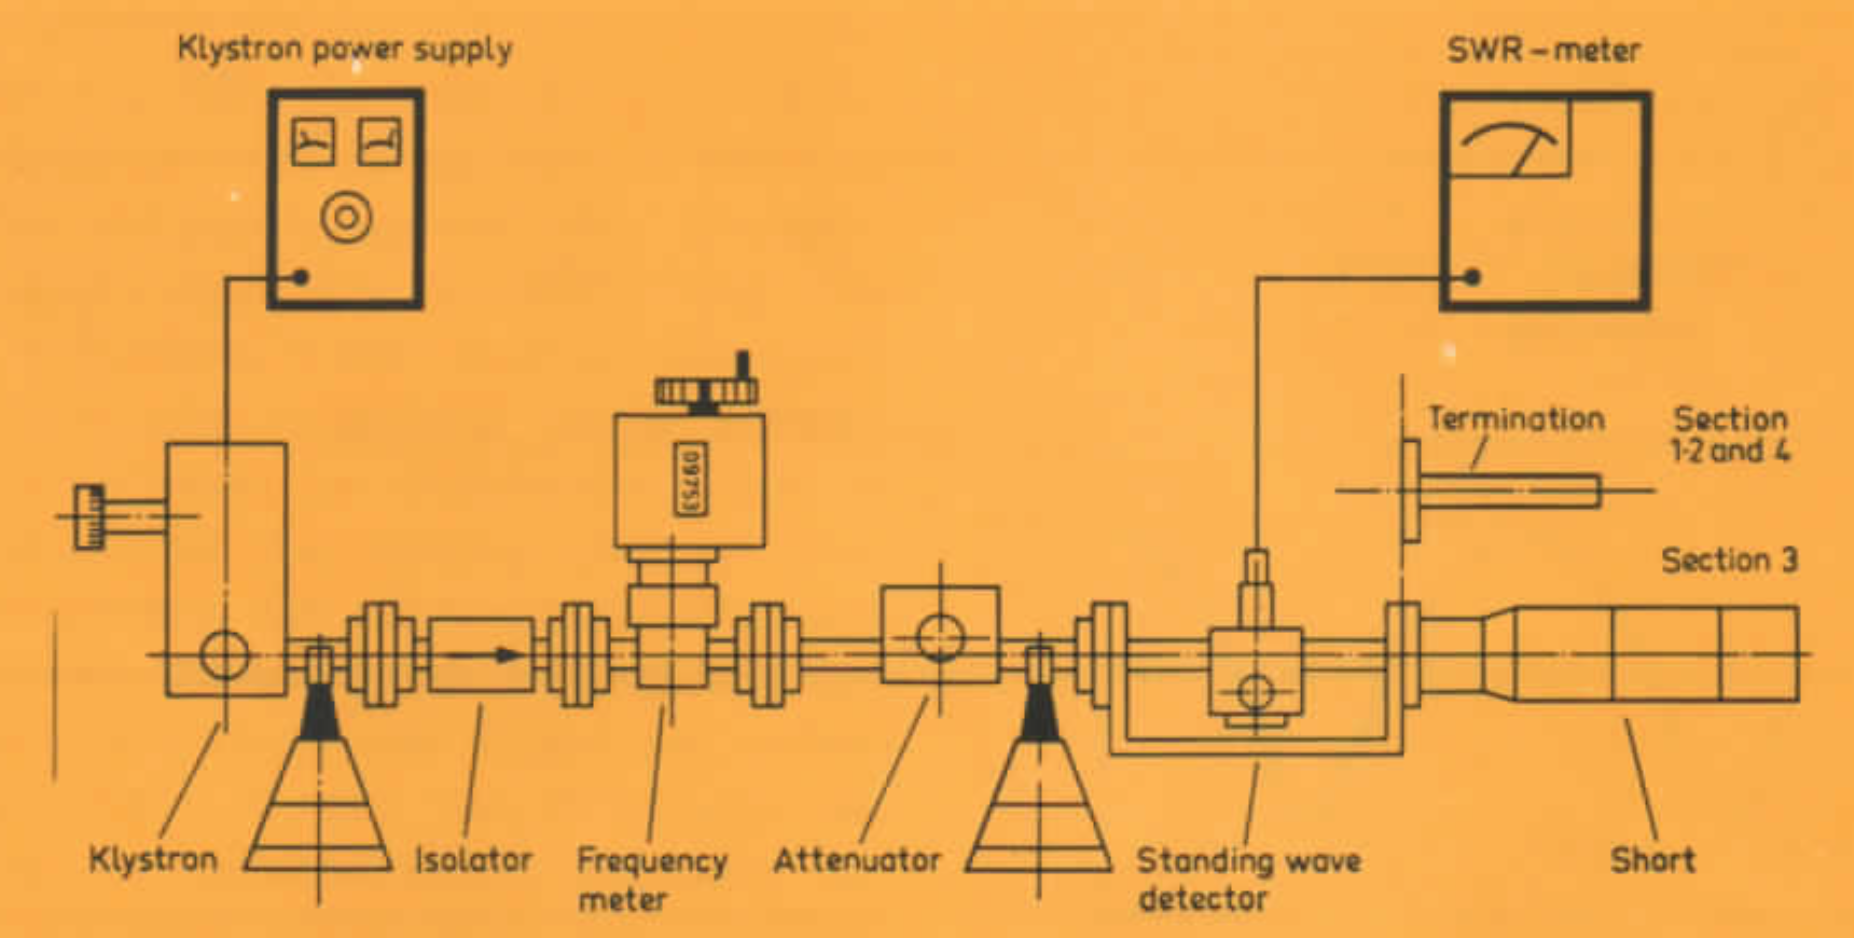
\includegraphics[width = 0.75\textwidth]{bilder/Aufbau_Teil2.png}
            \caption{Der Versuchsaufbau für die Messung von Frequenz, Wellenlänge und Dämpfung.}
            \label{fig:Teil2}
        \end{figure}
    \subsection{Untersuchung der Stehenden Wellen}
        Für den dritten Versuchsteil wird erneut der Stehwellendetektor verwendet, allerdings wird nun nach dem Detektor ein Bauteil eingebaut mit welchem man einen Stift mit variabler Tiefe an variabler Position in den Strahlengang einführen kann um eine Störung zu erzeugen.
        Der Hohlraum wird wieder durch einen Abschluss beendet.
        In diesem Versuchsteil werden drei Methoden verwendet um Stehende Wellen zu untersuchen, die direkte Methode, die ”\SI{3}{\decibel}-Methode” und die ”Abschwächer-Methode”.
        Die erste verwendete Methode ist die direkte bzw. SWR-Meter Methode.
        Bei dieser Methode wird ein Stift in den Strahlengang eingeführt und anschließend kann die Welligkeit direkt am SWR-Meter direkt abgelesen werden. Für größere Welligkeiten muss der Stift zu tief in den Strahlengang gebracht werden und es ist daher nötig auf die anderen Methoden zu wechseln um Störungen zu vermeiden.
        Die direkte Methode wird für Stifttiefen von \SI{3}{\milli\metre},\SI{5}{\milli\metre} und \SI{7}{\milli\metre} durchgeführt. Der Detektor wird dabei jeweils so platziert, dass auf dem SWR-Meter ein maximales Signal sichtbar ist und dieses wird anschließend auf \num{1.0} justiert. Für die Messung wird der Detektor in den Ort eines Minimums verschoben und der entsprechende Wert des SWR-Meters notiert.

        Für die \glqq \SI{3}{\decibel}-Methode\glqq  wird der Abstand zwischen zwei Punkten gemessen an denen die Detektor-Ausgangsspannung den doppelten Wert des Minimums erreicht. Über die folgende Formel lässt sich nun die Welligkeit bestimmen:
        \begin{equation}
            \label{eqn:SWR}
            S = \sqrt{1+\frac{1}{\sin^2\left(\frac{\pi \left(d_1 - d_2\right)}{\lambda_g}\right)}}
        \end{equation}
        Wobei $d_1 - d_2$ dem gemessenen Abstand entspricht.
        Für diese Methode wird der Stift mit \SI{9}{\milli\metre} in den Strahlengang gebracht und der Detektor in ein Minimum verschoben.
        Das SWR-Meter wird an diesem Minimum auf \SI{3}{\decibel} eingestellt und anschließend wird der Detektor einmal nach links und einmal nach rechts jeweils auf \SI{0}{\decibel} verschoben und die entsprechende Verschiebung wird notiert.

        Bei der \glqq Abschwächer-Methode\glqq  wird das Maximum am Detektor dem Minimum über Einstellen eines Dämpfungsgliedes gleichgemacht. Dadurch folgt für die Welligkeit die Formel
        \begin{equation}
            A_2 - A_1 = 20\cdot \log\left(S\right)
        \end{equation}
        Dabei sind $A_1$ und $A_2$ die Einstellungen des Dämpfungsglieds vor und nach der Anpassung.
        Auch bei der \glqq Abschwächer-Methode\glqq  wird eine Stifttiefe von \SI{9}{\milli\metre} verwendet.
        Die Sonde wird wieder auf den Punkt eines Minimums gebracht.
        Die Dämpfung wird nun auf \SI{20}{\decibel} eingestellt und das SWR-Meter erneut auf \SI{3}{\decibel} eingestellt.
        Der Detektor wird nun vertikal zum nächsten Maximum bewegt und anschließend die Dämpfung so angepasst dass das SWR-Meter erneut \SI{3}{\decibel} anzeigt.
        Die entsprechende Einstellung der Dämpfung wird notiert.
        \begin{figure}[H]
            \centering
            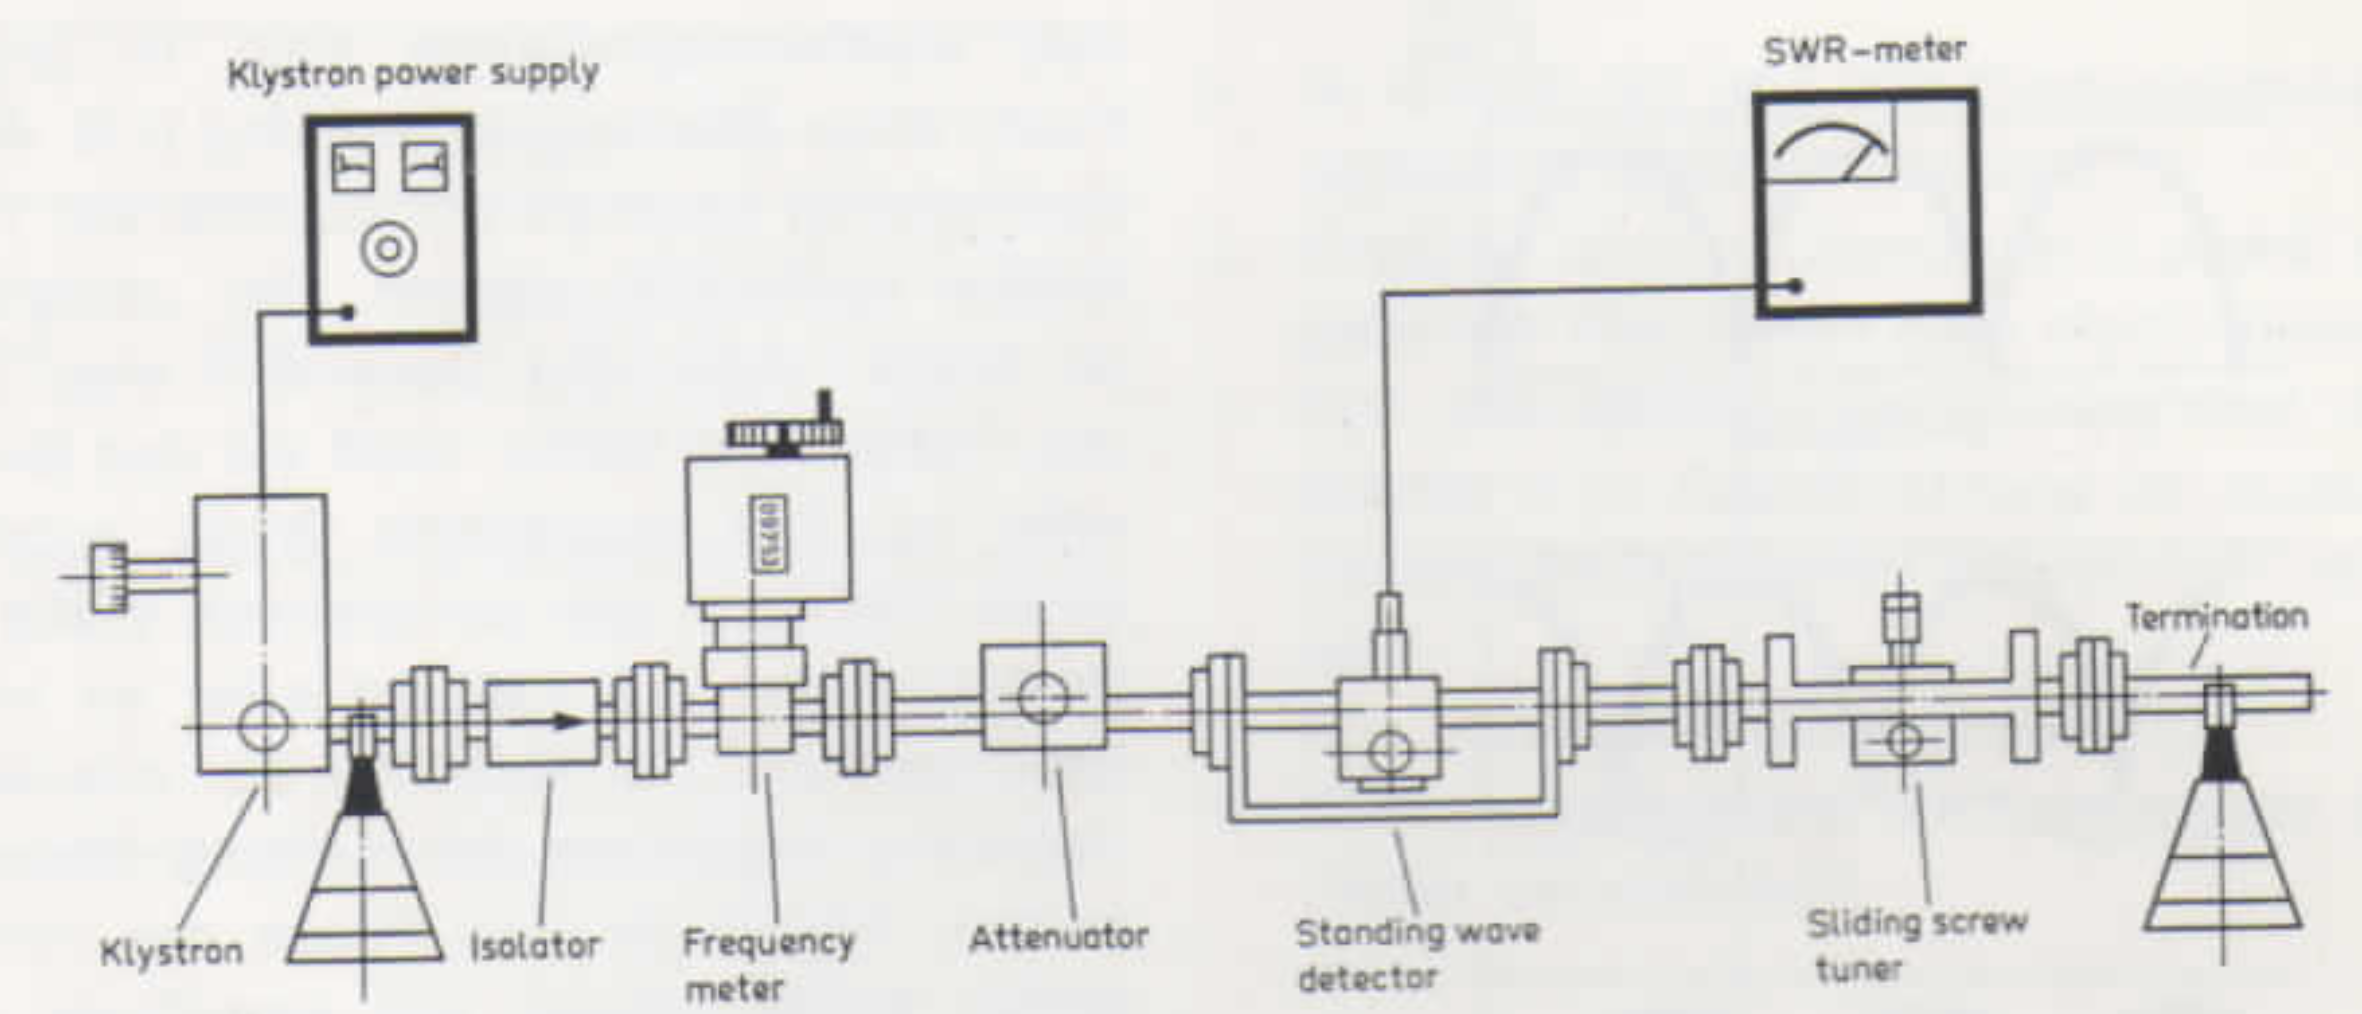
\includegraphics[width = 0.75\textwidth]{bilder/Aufbau_Teil3.png}
            \caption{Der Versuchsaufbau für die Untersuchung der Stehenden Wellen.}
            \label{fig:Teil3}
        \end{figure}